\section{Circuito per elettrocardiogramma (ECG) - 28.10.2014}

In questa esperienza costruiremo un circuito per effettuare un elettrocardiogramma (ECG).

\subsection*{Strumenti e materiali}

\begin{itemize} [noitemsep]
		\item Due pile da \SI{9}{\volt};
		\item Due elettrodi;
		\item Amplificatori operazionali OP07;
		\item Un integrato AD622 e un ISO124;
		\item Resistenze e capacità di vari valori;
		\item Paziente (umano).
\end{itemize}

\begin{wrapfigure}[19]{r}{0.24\textwidth}
\centering
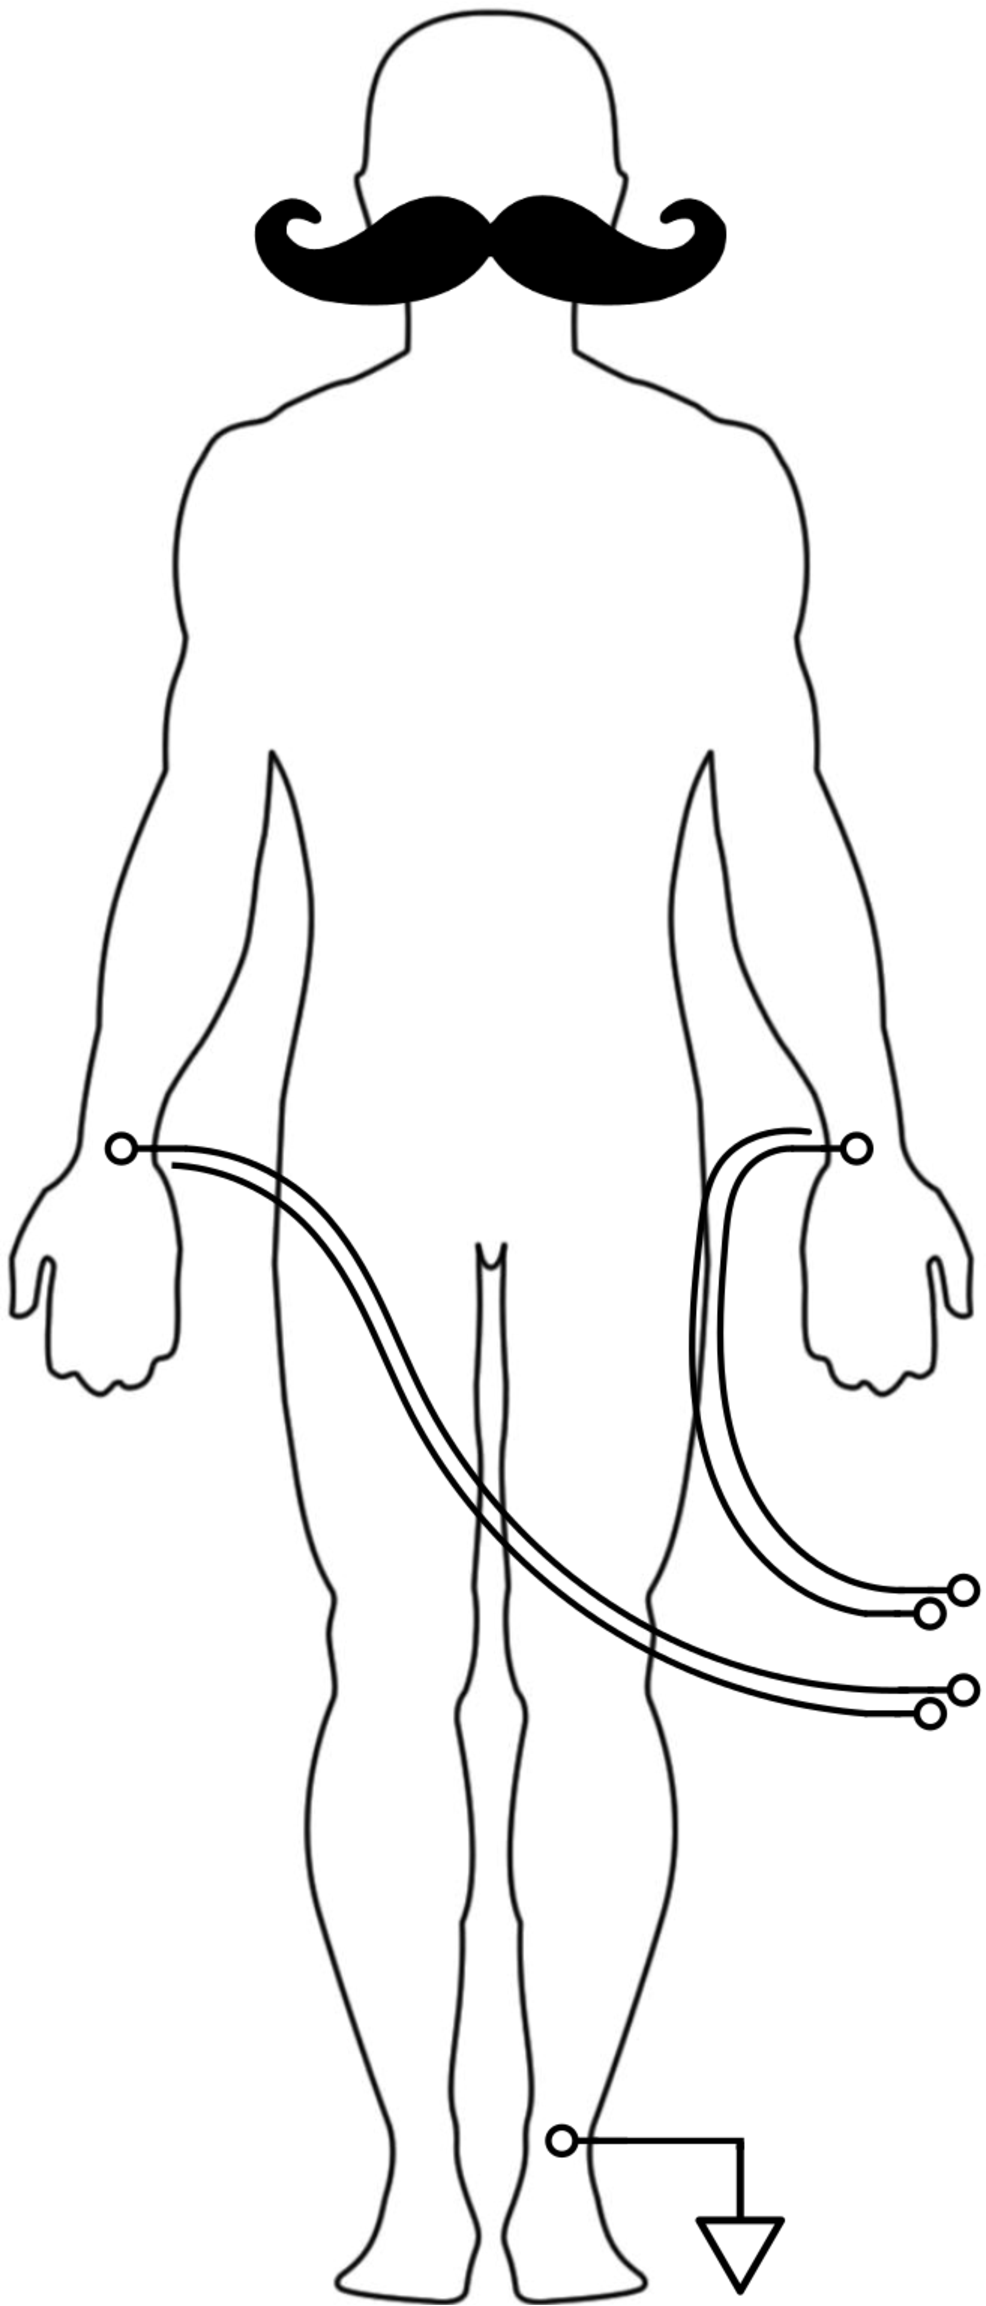
\includegraphics[width=.18\textwidth]{../E07/latex/mustache.pdf}%human.pdf}%doge.pdf}
\caption{Connessioni al corpo poco umano di uno degli sperimentatori.}
\label{fig7:human}
\end{wrapfigure}

\subsection{Premesse}

Per progettare un circuito che legga il segnale elettrico del nostro battito cardiaco a livello della cute, dobbiamo considerare che:
\begin{itemize} [noitemsep]
	\item Sulla superficie del corpo il segnale ECG è normalmente di circa \SI{1}{mV} (al massimo raggiunge i \SI{4}{mV}) ed ha una frequenza di circa \SI{1.25}{\Hz}.
	\item Gli elettrodi a nostra disposizione, che realizzano il collegamento tra la strumentazione e il corpo, creano un potenziale di circa \SI{700}{\mV}, quindi circa \num{200} volte maggiore del segnale cardiaco.
	\item Il segnale da misurare è piccolo, quindi dobbiamo porre particolare attenzione alle fonti di rumore elettromagnetico dati da effetti capacitivi e/o induttivi. Inoltre dobbiamo evitare che i cavi e il paziente si muovano durante la misurazione.
	\item È necessario che il paziente sia isolato dal lato di elaborazione del segnale, alimentato dall'alimentatore da banco, per evitare problemi di giri di massa.
\end{itemize}

Tenendo conto di ciò, nei paragrafi successivi analizzeremo gli aspetti legati all'abbattimento dei rumori e all'amplificazione del segnale in ingresso.

\subsection{Abbattimento dei rumori}

\subsubsection*{Operazionale U1}

Con il primo stadio in entrata (operazionale U1 in Figura \ref{cir7:elettro-cardiogramma}) eliminiamo i segnali di modo comune generati dagli elettrodi (oltre ad avere un'alta impedenza in ingresso e quindi un valore in entrata ad U1 più fedele alla reale ddp generata dal corpo). In testa ed in coda a questo stadio sono anche presenti delle capacità che creano due filtri: rispettivamente un passa basso ed un passa alto.

\paragraph*{Passa Basso}
Posto in testa ad U1, e composto dalle capacità $C_c$ e $C_d$, è necessario per abbattere eventuali rumori ambientali. Inserendo le capacito nel circuito come in Figura \ref{cir7:elettro-cardiogramma}, il datasheet dell'operazionale ci fornisce direttamente le frequenze di taglio di modo differenziale
\begin{equation*}
	\frac{1}{2 \pi R ( C_d + C_c ) } = \SI{194}{\Hz}
\end{equation*}
e di modo comune
\begin{equation*}
	\frac{1}{2 \pi R C_c} = \SI{4}{\kHz}
\end{equation*}

Con queste capacità riusciamo dunque ad eliminare i segnali di modo comune ad alte frequenze, ma soprattutto tagliamo ogni frequenza superiore ai \SI{200}{\Hz} in modo differenziale (il nostro segnale è infatti sui \SI{1.25}{\Hz} come da premesse), e dunque restringiamo drasticamente le frequenze ammesse ad essere amplificate dal nostro circuito.

\paragraph*{Passa Alto}
Essendo posto all'uscita dell'operazionale (capacità $C_1$ in Figura \ref{cir7:elettro-cardiogramma}), elimina eventuali segnali continui in output. La sua frequenza di taglio è di circa \SI{3}{\Hz}. Inoltre, è necessario che l'impedenza siano adattate, ovvero dovrà essere vista come infinita in entrata al prossimo blocco: per far ciò poniamo un ulteriore operazionale (un OP07, U2 in Figura \ref{cir7:elettro-cardiogramma}).

\subsubsection*{Operazionale U3 ed active gards}

Per diminuire l'effetto dei segnali di modo comune (dovuto agli elettrodi), è conveniente polarizzare in maniera uguale entrambe le calze dei cavi coassiali utilizzati per la connessione elettrodo-amplificatore. Così facendo il potenziale delle calze rimarrà uguale indipendentemente da eventuali movimenti dei cavi. Inoltre la differenza di potenziale fra la calza e il cavo che trasporta il segnale sarà minimizzata al fine di limitare le perdite sull'isolante.

Per effettuare la polarizzazione dobbiamo dunque attingere ad una tensione di $\approx \SI{700}{\milli\volt}$. Quindi abbiamo scelto di utilizzare la media fra i segnali entranti che, dato l'alto valore del segnale in modo comune, sarà la tensione desiderata. Infatti, se ricordiamo la struttura interna dell'amplificatore per strumentazione (Figura \ref{cir5:instr_amplif}), notiamo che, passando la stessa corrente sulle resistenze $R_1$ e su $R_G$, il punto ad $1/2 R_G$ è proprio a metà fra la due tensioni in ingresso.

\subsubsection*{Pile e amplificatore di isolamento}

Per alimentare il circuito abbiamo optato per utilizzare due pile da \SI{9}{\volt}, e come comune il polo positivo di una collegato al polo negativo dell'altra. Questo ha permesso di abbattere tutti i rumori relativi all'alimentazione dell'edificio e di avere una comune flottante rispetto a quella dell'oscilloscopio (in nero nella Figura \ref{cir7:elettro-cardiogramma}).

Per isolare ulteriormente il circuito ed evitare giri di massa abbiamo anche utilizzato un ISO124. Questo operazionale ha le seguenti caratteristiche
\begin{itemize}[noitemsep]
	\item Isola fino a \SI{1500}{\volt} e ammette una alimentazione da $\pm$ 4,5V a $\pm$ 18V;
	\item Possiede due alimentazioni separate e quindi anche due riferimenti di massa indipendenti l'uno dall'altro.
\end{itemize}

\begin{figure}[tpc]
\centering
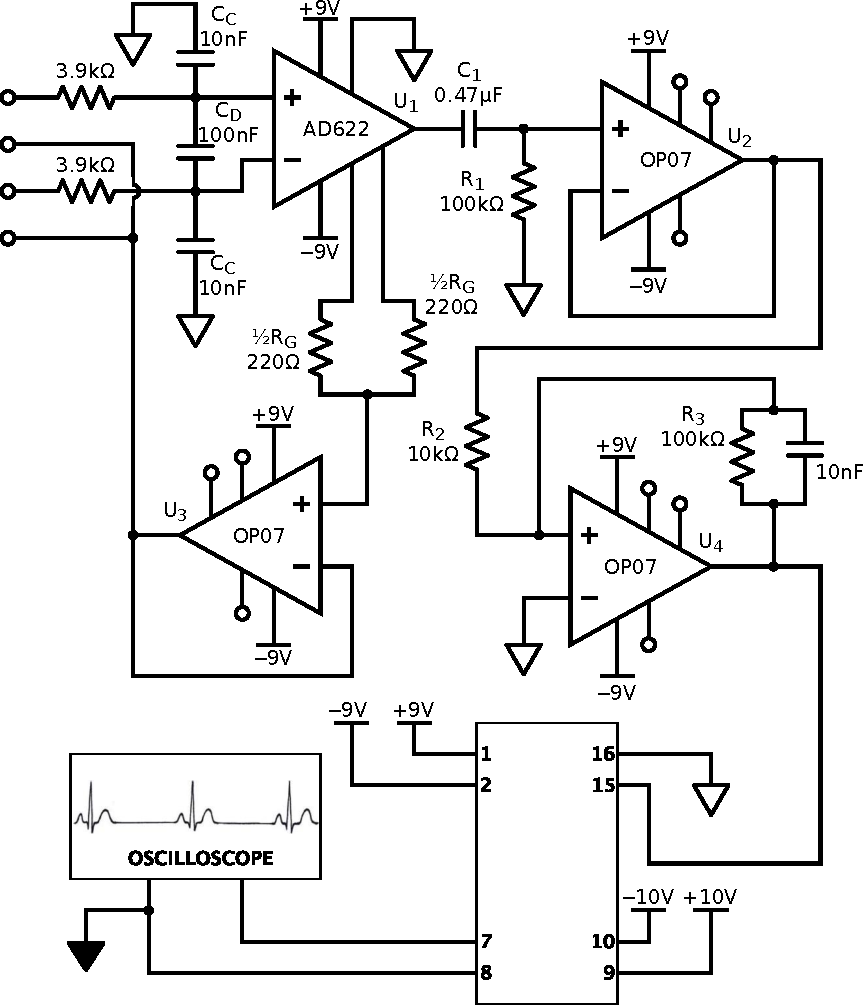
\includegraphics[width=.6\textwidth]{../E07/latex/circuito.pdf}
\caption{Schema del circuito da noi utilizzato per acquisire l'elettrocardiogramma. Il diverso colore della comune serve a rendere evidente l'indipendenza delle comuni fra il circuito e il collegamento all'oscilloscopio.}
\label{cir7:elettro-cardiogramma}
\end{figure}

\subsection{Amplificazione}

Dato il basso valore di tensione del segnale in entrata, abbiamo anche la necessità di amplificarlo per permettere alla strumentazione di leggerlo. Nel circuito ci sono tre stadi di amplificazione che amplificano il segnale di circa 800 volte.

\subsubsection*{Operazionale U1}
L'AD622, come visto nell'Esperienza 5, controlla l'amplificazione tramite la presenza di una resistenza posta nei punti dedicati della piedinatura (si faccia riferimento alla Figura \ref{cir5:ad622_ponte}). Con le resistenze utilizzate, l'amplificazione è data dalla legge (\ref{eq5:AD622_gain}) fornitaci dal costruttore
$$G_1=1+\frac{50.5 \si{\kilo\ohm}}{R_g} \approx 116$$

\subsubsection*{Filtro passa alto}
Con la sua frequenza di taglio di circa \SI{3}{\Hz}, il filtro passa alto in coda ad U1 riduce il nostro segnale (in uscita dal primo stadio di amplificazione dato da U1). Possiamo stimare di quanto viene ridotto considerando la funzione di partizione di un passa alto e facendone il modulo, ottenendo il guadagno. Vale dunque che
$$G_2=\frac{2 \pi R_1 C_1 \times \SI{1.25}{\Hz}}{\sqrt{1+(2 \pi R_1 C_1 \times \SI{1.25}{\Hz})^2}}\approx 0.35$$

\subsubsection*{Operazionale U4}
Questo operazionale è posto in un blocco con retroazione negativa non invertente. Dunque il suo guadagno è dato da
$$G_3=1+\frac{R_2}{R_3} \approx 11$$

L'amplificazione totale è dunque
$$G = G_1 \times G_2 \times G_3 \approx 450$$

La capacità di \SI{10}{\nano\farad} inserita è un ulteriore stadio di abbattimento dei rumori ad alte frequenze.

\subsection{Grafico dell'ECG}

Presentiamo ora in Figura \ref{fig7:ecg_output} l'elettrocardiogramma di uno degli sperimentatori.

\begin{figure}[htpc]
\centering
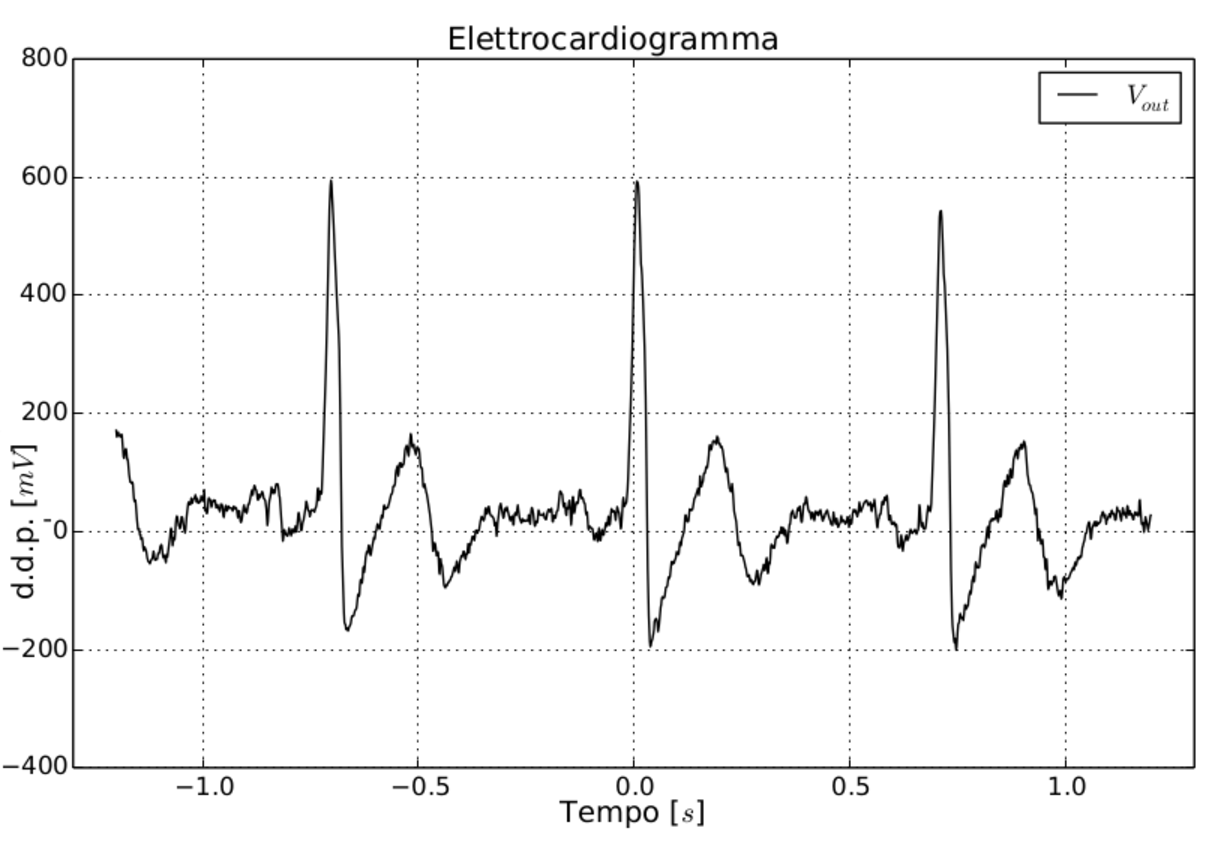
\includegraphics[width=.7\textwidth]{../E07/latex/g4.pdf}
\caption{Grafico della tensione registrata dall'oscilloscopio in funzione del tempo (ECG).}
\label{fig7:ecg_output}
\end{figure}

\subsection*{Conclusioni}
In questa esperienza siamo riusciti ad ottenere un elettrocardiogramma affetto da poco rumore, grazie agli stadi di abbattimento inseriti, e amplificato in maniera tale da poter essere letto facilmente dalla strumentazione.
